%--------------------------------------------------------------------------------------------------
% OBSERVACAO:
% 
% -> Arquivos que você pode editar:
%    - artigo.tex
%    - artigo_bibliografia.bib
%
% -> Arquivo .TeX codificado em UTF8                                                             
% -> Bibliografia em arquivo .bib (arquivo_bibliografia.bib)                                      
% -> Arquivo de imagens em .jpg, .eps ou .pdf
% -> Para compilar o TeX, execute 'compila_TEX.bat' (terminal do windows)
% 
% versão 1.1 - 19/05/2016
% versão 1.0 - 18/08/2015
%--------------------------------------------------------------------------------------------------
\documentclass{classe_cn}                 % Modelo <nao edite o arquivo classe_cn.cls>
\usepackage[brazil]{babel}                % Acentos
\usepackage[utf8]{inputenc}               % Codificação UTF8 (atenção aqui!)
\usepackage{graphicx}                     % Figura
\usepackage{amssymb}                      % Simbolos matematicos
\usepackage{color}                        % Cores
\usepackage{amsfonts}                     % Fontes
\usepackage{amsmath}                      % Fontes
\usepackage[fixlanguage]{babelbib}        % Acentos
\usepackage[normalem]{ulem}               % OK
\usepackage[retainorgcmds]{IEEEtrantools} % Formulas padrão IEEE
\usepackage{omlmathbf}                    % Simbolos Matematicos
\usepackage{epstopdf}                     % Figuras .eps
\usepackage{setspace}                     % Espaçamento flexível
\usepackage{cmap}                         % Mapear caracteres especiais no PDF
\usepackage{textcomp}                     % Funções e outros símbolos matemáticos
\usepackage{verbatim}                     % Pacotes verbatim
\usepackage{wrapfig}
%\usepackage{picins}
\startlocaldefs
\endlocaldefs

%--------------------------------------------------------------------------------------------------
% Inicio do Documento
%--------------------------------------------------------------------------------------------------
\begin{document}
\begin{frontmatter}        % Não alterar
\begin{fmbox}              % Não alterar
\dochead{Gerência da Informação} % Não alterar

%--------------------------------------------------------------------------------------------------
% Titulo do seu Trabalho
%   - pequeno bug (nao funciona cedilha)
%   - editar manualmente o cedilha na classe_cn.cls, linha 1015.
%--------------------------------------------------------------------------------------------------
\title{O Modelo de Crowdfunding}

%------------------------------------------------
% Informações sobre o autor #1
% - Ivete Maria Dias de Sangalo
%------------------------------------------------
\author[
  addressref = {ricardo1},                 % Identifica o autor #1
  email      = {ricardo.maia@ccc.ufcg.edu.br} % email para contato
]
{
  \inits{RdAM}      % Letras iniciais do autor #1
  \fnm{Ricardo de A.}  % Nome do autor #1 (first and middle name)
  \snm{Maia}   % Ultimo nome do autor #1 (last name)
}
%------------------------------------------------
% Informações sobre o autor #2
% - James Alan Hetfield
%------------------------------------------------
\author[
  addressref = {danielle2},                      % Identifica o autor
  email      = {danielle.vieira@ccc.ufcg.edu.br} % email para contato
]
{
  \inits{DdLV}       % Letras iniciais do autor #2
  \fnm{Danielle de L.}  % Nome do autor #2 (first and middle name)
  \snm{Vieira}    % Ultimo nome do autor #2 (last name)
}
%------------------------------------------------
% Informações sobre o autor #3
% - Freddie Bulsara Mercury
%------------------------------------------------
\author[
  addressref = {damiao3},                       % Identifica o autor
  email      = {damiao.domiciano@ccc.ufcg.edu.br} % email para contato
]
{
  \inits{DRD}      % Letras iniciais do autor #3
  \fnm{Damião R.} % Nome do autor #3 (first and middle name)
  \snm{Domiciano}    % Ultimo nome do autor #3 (last name)
}
%------------------------------------------------
% Informações sobre o autor #4
% - Virinha S. Dantas
%------------------------------------------------
\author[
  addressref = {lucas4},                 % Identifica o autor
  email      = {lucas.duarte@ccc.ufcg.edu.br} % email para contato
]
{
  \inits{LVD}     % Letras iniciais do autor #4
  \fnm{Lucas V.} % Nome do autor #4 (first and middle name)
  \snm{Duarte}     % Ultimo nome do autor #4 (last name)
}
%------------------------------------------------
% Informações sobre o autor #5
% - Virinha S. Dantas
%------------------------------------------------
\author[
  addressref = {adisio5},                 % Identifica o autor
  email      = {adisio.junior@ccc.ufcg.edu.br} % email para contato
]
{
  \inits{APFJ}     % Letras iniciais do autor #4
  \fnm{Adísio P. F.} % Nome do autor #4 (first and middle name)
  \snm{Júnior}     % Ultimo nome do autor #4 (last name)
}

%------------------------------------------------
% Endereço dos autores
%------------------------------------------------
\address[id=ricardo1]{
  \orgname{Universidade Federal de Campina Grande,
           Centro de Tecnologia e Recursos Naturais,
           Unidade Acadêmica de Engenharia Civil},
  \street{Rua Aprígio Veloso, 882, Bairro Universitário},
  \postcode{58429-140},
  \city{Campina Grande},
  \cny{Brasil.}
}

\end{fmbox}

%--------------------------------------------------------------------------------------------------
% Resumo do Trabalho
%--------------------------------------------------------------------------------------------------
\begin{abstractbox}
	
\begin{abstract} 
Com o surgimento de novas tecnologias, tornando a comunicação instantânea e eliminando as restrições geográficas, novas oportunidades surgiram para aqueles que pretendem investir em uma boa ideia, seja ela um novo produto, projeto socioambiental, ou mesmo de cunho cultural. O crowdfunding entra neste cenário como uma ferramenta que permite arrecadação de recursos e facilita a interação entre empreendedores e investidores de uma forma mais democrática. Assim, este trabalho busca fazer um pequeno levantamento sobre o modelo do crowdfunding, levando em consideração sua definição e suas práticas, além de descrever de forma sucinta algumas plataformas e projetos de destaque no Brasil e no mundo, possíveis graças ao financiamento coletivo.
\end{abstract}

%--------------------------------------------------------------------------------------------------
% Palavras-chaves: Entre 3 e 6 palavras chaves
%--------------------------------------------------------------------------------------------------
\begin{keyword}
  \kwd{Financiamento coletivo}
  \kwd{Internet}
  \kwd{Inovação}
\end{keyword}

\end{abstractbox} % Não alterar
\end{frontmatter} % Não alterar

%--------------------------------------------------------------------------------------------------
% Escreva o seu artigo!
%--------------------------------------------------------------------------------------------------

%------------------------------------------------
% Seção 1
%------------------------------------------------
\section{Introdução}
O investimento em ideias é um tabu, que necessita passar por vários estágios burocráticos. As ideias devem ser apresentadas para as empresas, caso seja do interesse delas (gerando lucros) elas investirão nessa ideia. Por essa razão muitas ideias que são do interesse comum, projetos culturais sem fins lucrativos, não são interessantes para grande parte das industrias.

O Crowdfunding conseguiu modificar esse senário, pois, ele permitiu que essas ideias chegassem ao público. Basicamente o Crowdfunding é uma plataforma (não necessariamente com este nome) que permite o cadastro de campanhas para arrecadar recursos para o desenvolvimento de projetos.

\begin{quote}
“O crowdfunding cultural funciona da seguinte maneira: um grupo de pessoas é estimulado por um proponente, que inscreve seu projeto em uma plataforma de online, a investir pequenas ou médias parcelas de dinheiro a fim de alcançar um determinado orçamento, mais amplo, que objetiva viabilizar a execução de uma ação de cunho artísticocultural.”\cite[p. 3]{SEQUEIRA:sd}
 \end{quote}

Desta forma permitindo que um novo mercado surja, dando novas oportunidades, tanto para os idealizadores quanto para os beneficiados. Essa facilidade ocorre por meio dos benefícios que a internet trouxe para o homem contemporâneo, aproximando virtualmente a população mundial para contribuir para novos projetos que os instiguem a empatia. Segundo Felinto \cite{FELINTO:2012} sendo um processo que o próprio público financia um projeto através de sites da internet, promovendo para um filme, obra de arte ou produto de qualquer espécie.

Depois dessa compreensão, será demonstrado como podemos iniciar uma campanha através das ferramentas online de financiamento coletivo, que consistirá em quatro passos: a ideias, que é o início de todo o processo, onde o idealizador ou grupo possui uma ideia inicial que possui propriedades para desenvolver; O planejamento, que permitirá o crescimento e objetivos que serão alcançados; A arrecadação, qual ferramenta será usada para conseguir a quantidade necessária para pôr no mercado, ou apenas finalizar, o projeto idealizado e por último o processo de divulgação. Que chegará ao público alvo, que investirá no projeto.

Os benefícios são inúmeros como a comprovação de mercado, que consegue encontrar um padrão na preferência do público. Produção sobre demanda, que diminui a produção exagerada de produtos, entre outros que serão abordados ao decorrer deste artigo. Mas o Crowdfunding não possui apenas benefícios, que são o fracasso da campanha ou o mal-uso do dinheiro investido, que gerará consequências para o site e o idealizador do projeto.

A grandes ferramentas mundiais de financiamento coletivo como o Kickstarter que, “No ano de 2012, através do Kickstarter a cantora Amanda Palmer conseguiu arrecadar 1.2 milhões de dólares para gravar seu CD, conseguindo dez vezes mais do que o valor que o projeto pedia. ” \cite[p. 9]{CAVALCANTI:2013}, sendo uma ferramenta muito poderosa para angariar recursos. O Brasil possui plataformas de Crowdfunding, algumas que possuem um nicho específico De projetos, como o Catarse que foi o “primeiro endereço eletrônico que apresentou a plataforma de crowdfunding, voltada somente para projetos culturais” \cite{COCATE:2012}.

Em escala mundial há vários projetos bem sucedidos que forma financiado através de plataformas do Crowdfunding, como filmes, games, podcasts, livros, HQs e eventos, que serão abordados ao decorrer desse artigo.

Trabalharemos esses conceitos ao decorrer desse trabalho, abordando de forma mais aprofundada o conceito de Crowdfunding, as plataformas que utilizam esse sistema de arrecadação de recursos, seus acertos e erros tanto quanto os projetos que surgiram através dessa grande ferramenta.

%------------------------------------------------
% Seção 2
%------------------------------------------------
\section{Criação de campanha crowdfunfing}

Em primeiro lugar, é preciso escolher um bom motivo pelo qual esta fazendo a campanha para que convença as pessoas a apoiar o seu projeto. Pois um motivo muito fraco pode não convencer os investidores a apoiarem o projeto. Apresentando a ideia de forma clara, explicando a trajetória do projeto, dizendo o porquê dele ser importante para você e ou a sociedade, mostrando o que você pretende alcançar com a campanha.

O titulo é o primeiro encontro dos futuros contribuintes da campanha. Portanto ela deve ser explicada em poucas palavras qual o objeto da campanha e ao mesmo tempo sendo chamativa ao leitor, para que ele se convença a investi no projeto.

Oferecer uma recompensa para que as pessoas invistam no seu projeto pode ser uma boa ideia, oferecendo vantagens para certos valore investidos, para quanto mais for investido maior será os benefícios da pessoa que esta disposta a investi. Fornecer uma recompensa não é obrigatório, porém pode fazer muita diferença nos valores arrecadados para sua campanha, pois muitas pessoas investem por acreditarem no projeto e outras pelas recompensas oferecidas.

Antes de começar uma campanha de financiamento coletivo é bom saber o valor mínimo do orçamento para que seu projeto aconteça, deixando uma pequena margem para imprevistos, tentando escolher um orçamento mais realista possível.

Divulgar o máximo possível sua ideia é essencial, uma vez que quanto maior o alcance dela maior será a chance de ter pessoas dispostas a investi nela, e mesmo que não invistam elas podem se sensibilizar e acabar compartilhando sua ideia para que outras vejam, aumentando cada vez mais o alcance do seu projeto. \cite{XAVIER:2016}
%------------------------------------------------
% Seção 3
%------------------------------------------------
\section{Forças do modelo crowdfunding}

Por ser uma plataforma muito conhecida no mercado, pessoas que você nunca viu iram investi em sua campanha, podendo essa pessoa ser da sua cidade ou do outro lado do mundo, pois elas se identificaram com o objetivo da sua campanha ou se interessaram por alguma das recompensas oferecidas.

Um dos principais benefícios para quem coloca um projeto em uma campanha de crowdfunding é a comprovação de mercado. Uma vez que esse tipo de financiamento se tornou bastante atraente ultimamente para investidores, e também um bom projeto pode aumentar a reputação do autor do projeto.

Outro benefício do crowdfunding vem do fato de permitir saber exatamente quantos produtos deverão ser fabricados em uma primeira tiragem ou versão, já que só quem pagou receberá o item. \cite{PEREIRA:2016}

%------------------------------------------------
% Seção 4
%------------------------------------------------
\section{Fraquezas do modelo de crowdfunding}

O modelo está sujeito a fatores que podem desmotivar usuários. Como o não alcance da meta do orçamento do projeto na campanha, o mau uso do dinheiro obtido na campanha por partes dos donos dos projetos, entregas de produtos de baixa qualidade e atraso na entrega do produto em relação ao prazo estabelecido na campanha. \cite{PEREIRA:2016}

Outro fator que pode contribuir para o fracasso do financiamento é uma meta ou uma ideia muito ousada. Como por exemplo, o Smartphone Ubuntu Edge, que não alcançou a meta ousada de arrecadar mais de US\$ 32 milhões \cite{GAZETA:2017}

%------------------------------------------------
% Seção 5
%------------------------------------------------
\section{As plataformas de financiamento coletivo}

O crowdfunding, como já foi se tratado acima, também chamado financiamento coletivo, consiste em conseguir recursos financeiros para financiamento de um projeto a partir de doações de outras pessoas, logo abaixo será citada empresas brasileiras e estrangeiras, que conseguiram através de muitos projetos arrecadar valores impressionantes.

\subsection{Plataformas nacionais}

\subsubsection{Catarse}

Plataforma Catarse, segundo seu site que está disponível para que pessoas possa colocar seus projetos, para que possa encontrar apoiadores para o mesmo. Ela foi criada em 2011, desde seu começo até os dias atuais ela tem em seus históricos cerca de 2 mil projetos financiados por 241 mil apoiadores, tendo um lucro aproximadamente de 35 milhões arrecadado e atendendo tipos variado de projeto, diante desses valores e informações faz com que a plataforma Catarse seja a mais popular no Brasil.

A taxa administrativa da Catarse é de “13\% para campanhas de crowdfunding Flexíveis e também para campanhas Tudo ou Nada que alcançarem ou superarem a meta.” \cite{BRASIL:2017}. Até o final de 2015, a empresa adotava a postura de “tudo ou nada”, ou seja, se o projeto não atingisse a meta de orçamento, os usuários recebiam de volta todo o dinheiro que investiram. Entretanto, agora há o Catarse Flex, que permite que o arrecadador fique com aquilo que conseguir.

\subsubsection{Kickante}

A Kickante criada em 2013, atualmente é umas das principais empresas quando se fala em arrecadação em dinheiro, tendo seu “Site recorde de arrecadação de crowdfunding na América Latina. Mais de 50.000 campanhas lançadas, captando mais de R\$ 40 milhões em colaborações.” \cite{BRASIL:2017}.

Tendo sua plataforma mais voltada para questão socail. “Aqui na Kickante, nós somos apaixonados pela cultura, causas sociais e empreendedorismo. Amamos tudo que faz uma grande diferença em nosso país, projetos grandes e pequenos que influenciem de alguma maneira a nossa comunidade.” \cite{KICKANTE:2017}. O Kickante tem como diferencial aceitar contribuições parceladas pelo cartão de crédito.

Em relação a sua taxa administrativa, “Menor Taxa do Mercado (e oferecemos assessoria gratuita). 12\% para projetos que alcançarem ou superarem a meta (Flexível ou Tudo ou Nada). Porém, se sua campanha de crowdfunding for Flexível e você não alcançar a meta, a taxa é de 17,5\%. Já inclusas as taxas cobradas pelos meios de pagamento.”  \cite{BRASIL:2017}.

\subsubsection{Vakinha}

Apesar de não parecer mais a Vakinha seja a empresa mais velha no mercado das plataformas de financiamento coletivo, ela foi criada em 2006, “A ideia do Vakinha surgiu em 2006, no casamento do sócio-fundador, Luiz Felipe Gheller, quando o Fabrício Milesi, atual CEO da empresa, ficou encarregado de arrecadar os presentes na forma de dinheiro, algo cada vez mais comum nos dias de hoje.” \cite{VAKINHA:2017}. Já que não consegui ele, se junto com os mais 3 membro da empresa, para pode expandir a empresa para internet. Então foi em 2009 que, “Em janeiro de 2009, o Vakinha foi lançado com uma proposta muito simples: levar a prática de fazer uma vaquinha para a internet. Esse conceito, com o lançamento e sucesso do Kickstarter, nos Estados Unidos, ficou posteriormente conhecido como crowdfunding (apesar das diferenças que preservamos no nosso modelo).”

Finalmente, em 2013, o Vakinha atingiu o ponto de equilíbrio, sem mais necessidade de nenhum aporte dos investidores que sempre estiveram presentes quando necessário (e não foram poucas vezes!). Em 2015 o Vakinha enfim lançou sua nova plataforma, desenhada desde 2013, com uma série de ferramentas planejadas especificamente para esse novo mercado, incluindo grandes diferenciais: ferramentas de antifraude própria e negociação com meios de pagamentos que permitiram ao site ter as taxas mais baixas do mercado. “Atualmente o Vakinha é o maior site do gênero no país, com mais de 400 mil vaquinhas abertas e mais de 20 milhões de reais arrecadados. Hoje, a empresa atua com uma equipe que envolve 12 pessoas.” \cite{VAKINHA:2017}.

\subsection{Plataformas estrangeiras de Crowdfunding}

Diante de valores tão grande ficamos com supresso com esses valores, mas esses valores são pequenos quando falamos das empresas estrangeiras de Crowdfunding. Abaixo segue alguns exemplos de plataformas estrangeiras.

\subsubsection{Kickstarter}

Então a Kickstarter a maior empresa de financiamento do mundo, fundada em 2008, “Criado por cinco amigos norte-americanos, o site reúne diversas idéias criativas de pessoas do mundo inteiro, e a variedade dos projetos é imensa: vão desde tecnologia, design, arte, música e vários outros.” \cite{CANALTECH:2017}

São mais de 2,4 bilhões de dólares arrecadados ao longo de 5 anos para mais de 106 mil projetos. Entre eles os famosos Óculos Rift (comprado posteriormente pelo Facebook) e até o filme baseado na série The Veronica Mars (que arrecadou mais de 5 milhões de dolares em sua campanha).

\subsection{Indiegogo}

Indiegogo é um site de financiamento coletivo internacional fundado em. Sua sede fica na Califórnia. O site é um dos primeiros sites a oferecer financiamento coletivo.

Em 2014, o Indiegogo lançou Indiegogo Life, um serviço que as pessoas podem usar para arrecadarem dinheiro para emergências, despesas médicas, comemorações, ou outros eventos de vida. O Indiegogo vida não cobra uma taxa de plataforma, de modo angariadores de fundos mantem mais do dinheiro que eles levantam.

\subsection{Rockethub}

Fundado em 2009 em Nova York, o Rockethub é um tipo de plataforma de crowdfunding que inicialmente atendia mais a projetos de tecnologia e ciência, no entanto, com o passar do tempo ele foi se transformando em um sistema mais aberto voltado a projetos educacionais que já atendeu a dezenas de milhares de instituições ao redor do mundo.

Além de ajudar a milhares de empreendedores ao redor do mundo, o financiamento coletivo também tem feito à diversão de muitos apoiadores por aí, seja através de games, discos e até filmes extremamente interessantes.

%------------------------------------------------
% Seção 6
%------------------------------------------------
\section{Ideias que já ganharam vida com esse modelo de negócio}

\subsection{Pebble Time}

O maior e mais rapida campanha de financiamento coletivo, \$20,338,986 arrecadados até hoje 24/07/2017, além de ser um dos primeiros smartwatch do mercado, ele tem como chamativo ser mais um relógio do que smartwatch, com interações mais simples com o usuário, design mais parecido com um relógio tradicional, bateria que dura mais de uma semana e preço atraente. \cite{ONOFFRE:2017}

\subsection{OUYA}

Um dos projetos que popularizou o Kickstarter, o OUYA se propunha ser um vídeo-game minúsculo, usando android e rodando jogos tanto da Google Play como de sua biblioteca própria. O projeto recebeu até a data de 24/07/1017  \$8,596,474. Porem sua relevância no Mercado diminuiu bastante depois de aparelhos concorrentes mas potentes e com bibliotecas mais atraentes surgiram no mercado como Nvidia Shield e SmartTVs com Android. \cite{ONOFFRE:2017}

\subsection{Bloodstained: Ritual of the Night}

Bloodstained é um jogo com uma história em particular. O Seu criador Koji Igarashi, é considerado um dos super produtores de jogos japoneses responsável por um dos maiores sucessos da KONAMI  e sua aclamada franquia de jogos Castlevania, o Castlevania sinfony of de night que mesmo sendo um jogo 2D com sprites foi um dos maiores sucessos da quinta geração de consoles onde somente os jogo 3D reinavam. Em 2015 Koji Igarashi saiu da KONAMI e abriu uma campanha no Kickstarter para a criação do jogo Bloodstained, que usa as mesmas mecânica  e atmosfera de Castlevania sinfony of de night, sendo assim um “continuação espiritual” da mesma. Atualmente o jogo já arrecadou \$5,545,991 e ainda não foi lançado. \cite{ Velberan:2017}

\subsection{Mighty No. 9}

Um do projeto mais controversos do Kickstarter, Mighty No. 9 tem um historio parecida com a de Bloodstained: Ritual of the Night. Criado por Keiji Inafune que saiu da Capcom, tinha como objetivos se uma “sequencia espiritual” de sua outra criação MegaMan, o projeto arrecadou \$3,845,170, porem suas vendas foram prejudicadas por muitas críticas dos financiadores e da comunidade de jogadores, entras as críticas estão: os constantes adiamentos do lançamento, o aumento excessivo da meta de arrecadação e a qualidade inferior do jogo em relação ao que foi prometido.

%------------------------------------------------
% Seção 7
%------------------------------------------------
\section{Mercado mundial}

Com a globalização da economia através, principalmente, das inovações tecnológicas que permitem maior facilidade e agilidade nas comunicações, o mercado precisa se adaptar constantemente e se integrar à essas inovações para manter sua capacidade de atender à crescente demanda e de sobreviver a intensa competitividade, uma vez que seus concorrentes podem estar em qualquer parte do mundo.

Como visto anteriormente neste trabalho, o modelo do crowdfunding surgiu como uma ferramenta que permite incorporar essas inovações tecnológicas à prática econômica, permitindo que projetos individuais ou de pequenas e médias empresas, que geralmente possuem maior dificuldade de acesso ao crédito por meios convencionais, como bancos, possam ser desenvolvidos.

Assim, o crowdfunding é visto como uma forma mais democrática de economia, tanto em relação a quem está empreendendo, como também em relação aqueles que investem. Não existe a necessidade de haver disponível um grande capital para participar como investidor em algum projeto pois, uma vez que há um grande número de indivíduos agindo coletivamente em prol de um interesse comum, os valores a serem investidos se tornam menores e mais dependentes da vontade e capacidade de doação do investidor, mesmo que o valor a ser arrecadado seja consideravelmente alto. Uma pesquisa divulgada pelo SEBRAE \cite{SEBRAE:2017} e realizada pelo Catarse em parceria com a Chorus, no período 2013/2014 é um bom indicativo deste comportamento. A pesquisa aponta que no Brasil 64 \% das pessoas que participam do financiamento coletivo ganham até 6 mil reais por mês, sendo que pessoas com mais escolaridade e em uma faixa etária de 25 a 30 anos são as que possuem maior participação.

Andrade \cite{ANDRADE:2017} descreve que atualmente, o crowdfunding é praticado em mais de 160 países, segundo o relatório do The Crowdfunding Centre. Em 2014 foram arrecadados cerca 16,2 bilhões de dólares no mundo por meio do crowdfunding, um aumento de 167 \% em relação ao ano anterior, com uma arrecadação de 6 bilhões de dólares \cite{PASCOAL:2017}. No entanto, está fenômeno que se apresenta bastante difundido em outros países, como os Estados Unidos, ainda não possui grande expressividade no Brasil. Um exemplo disso, é o fato de apenas em 2015 o valor de arrecadações a nível mundial por meio do financiamento coletivo girar em torno de 9,4 bilhões de dólares, enquanto que no Brasil os 32 milhões de reais movimentados pelo Catarse em seus quatro anos de funcionamento, representam apenas 0,1 \% desse total \cite{ALVES:2017}.

Apesar disso, a população brasileira possui um forte caráter empreendedor, característica marcante principalmente em cenários como o atual com uma alta taxa de desemprego, onde o financiamento coletivo por ser menos burocrático e mais viável do que outras formas de financiamento, desponta como uma alternativa bastante interessante. Assim, espera-se que este tipo de prática cresça no país nos próximos anos, como ocorreu e ocorre em outros países. Vale a ressalva que campanhas com intuito social e/ou ambiental também possuem um forte apelo entre as campanhas nacionais.

%------------------------------------------------
% Seção 10
%------------------------------------------------
\section{Considerações Finais}

Como podemos compreender, através do texto acima, o crowdfunging possibilita o desenvolvimento de várias ideias que dificilmente conseguiriam alcançar o público com tanta clareza e rapidez. Essa “nova” abordagem do mercado de investimento proporcionou um grande aumento em projetos que antes não receberiam investimentos, através dos métodos tradicionais que é a apresentação do projeto para as empresas investirem nele. Como as empresas visam mais o seu lucro ou alguma forma de gerar marketing de seu produto para lucrarem, os projetos que elas investiriam seriam aqueles que suprissem suas necessidades. Assim, deixando projetos com características culturais ou ambientais, que não traria retorno lucrativo, eram deixados de lado, empobrecendo e desestimulando esse tipo de iniciativa.

Com a ideia de financiamento foi possível quebrar esse paradigma que impedia o investimento em projetos culturais. Com o público final podendo contribuir para ter acesso a projetos que os beneficiassem culturalmente. E não só os projetos culturais. Através dessa nova forma de arrecadação de recursos abriu um novo mercado de empreendedores que possuem ideias de proporções pequenas, mas também de ideias que não pareceriam interessantes para as indústrias, mas que deram muito certo depois de alcançarem suas metas e desenvolverem seu produto.

Com uma maior facilidade de iniciar uma campanha na plataforma de financiamento coletivo, e sua forma de divulgação podendo ser através dá própria plataforma. Mas, as redes sociais também facilitam muito essa divulgação, atraindo cada vez mais pessoas e startup com novas ideias para esse tipo de arrecadação de recursos.

%--------------------------------------------------------------------------------------------------
%--------------------------------------------------------------------------------------------------
% Define o arquivo BIB (bibliografia)
%--------------------------------------------------------------------------------------------------
%--------------------------------------------------------------------------------------------------
\bibliographystyle{bmc-mathphys}   % NAO EDITAR!
\bibliography{artigo_bibliografia} % NAO EDITAR! - Bibliography file (usually '*.bib' )

\vspace{1.0cm}

\begin{table}[h!]
\centering
\begin{tabular}{lp{8cm}}
 \raisebox{-\totalheight}{
\includegraphics[width=0.3\textwidth, height=50mm]{f1.jpg}} &  
  \vspace{0.1cm} Ricardo de Andrade Maia nasceu em Catolé do Rocha, interior do estado brasileiro Paraíba. Atualmente é
  graduando em Ciência da Computação pela Universidade Federal de Campina Grande (UFCG) e está
cursando o quarto semestre. Tem grande interesse em pesquisa na área de Desevolvimento Mobile e Desevolvimento de Games\\
  \raisebox{-\totalheight}{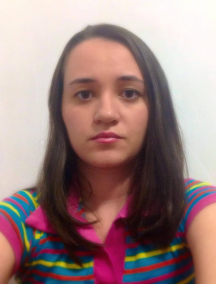
\includegraphics[width=0.3\textwidth, height=50mm]{f2.jpg}} &  
  \vspace{0.1cm} Danielle de Lima Vieira nasceu em Catolé do Rocha no estado da Paraíba. Atualmente é
  graduando em Ciência da Computação pela Universidade Federal de Campina Grande (UFCG) e está
cursando o quarto semestre. Tem grande interesse em pesquisa na área de Mobile e Desevolvimento, Desevolvimento de Games e computação grafica 3d. \\
  \raisebox{-\totalheight}{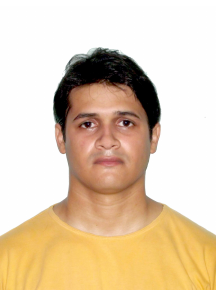
\includegraphics[width=0.3\textwidth, height=50mm]{f3.jpg}} &  
  \vspace{0.1cm} Damião Robson Domiciano 29 de Janeiro de 1988 em Santa Luzia, interior do estado brasileiro Paraíba. Atualmente é
  graduando em Ciência da Computação pela Universidade Federal de Campina Grande (UFCG) e está
cursando o terceiro semestre. Tem grande interesse em pesquisa na área de Análilse de Dados (AD).  \\
  \raisebox{-\totalheight}{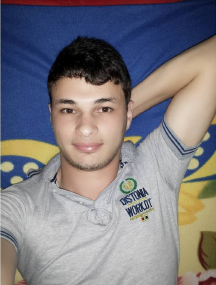
\includegraphics[width=0.3\textwidth, height=50mm]{f4.jpg}} &  
  \vspace{0.1cm} Lucas Venancio Duarte 14 de Novembro de 1996 em Alagoa Nova, interior do estado brasileiro Paraíba. Atualmente é
  graduando em Ciência da Computação pela Universidade Federal de Campina Grande (UFCG) e está
cursando o terceiro semestre. Tem grande interesse em pesquisa na área de Inteligência artificial (IA). \\

\end{tabular}
\end{table}

\begin{table}[h!]
\centering
\begin{tabular}{lp{8cm}}
\raisebox{-\totalheight}{
\includegraphics[width=0.3\textwidth, height=50mm]{f5.jpg}} &  
  \vspace{0.1cm} Adísio Pereira Fialho Júnior nascido no dia  22 de Janeiro de 1995 na cidade Cuité, interior do estado brasileiro Paraíba.
  Atualmente esta graduando em Ciência da Computação pela Universidade Federal de Campina Grande (UFCG) e está
  cursando o quarto semestre. Tem grande interesse em pesquisa na área de PERÍCIA COMPUTACIONAL.\\
\end{tabular}
\end{table}

%\end{tabular}
%\end{table}

%--------------------------------------------------------------------------------------------------
% FIM DO ARTIGO
%--------------------------------------------------------------------------------------------------
\end{document}
